\chapter{Visualização e Análise de Dados}

\section{Visualização centralizada no Grafana}

A visualização dos dados de telemetria assume um papel crucial para a compreensão e monitorização eficaz de sistemas distribuídos. Embora as ferramentas Prometheus, Jaeger e Loki disponham de interfaces próprias para análise independente de métricas, \textit{traces} e \textit{logs}, a fragmentação das informações pode dificultar a correlação rápida entre estes dados. Por esse motivo, optou-se pelo Grafana como camada de visualização unificada, visando uma experiência integrada e eficiente. Entre as principais vantagens da utilização do Grafana destacam-se:

\begin{itemize}
\item a centralização das métricas, \textit{logs} e \textit{traces} num único painel interativo;
\item a capacidade avançada de correlação entre diferentes tipos de dados, facilitando a identificação de causas-raiz em anomalias;
\item a configuração unificada de alertas abrangendo todas as fontes de dados;
\item a interface intuitiva e personalizável, acessível a diferentes perfis técnicos;
\item linguagens de consulta especializadas (\textit{PromQL}, \textit{LogQL}) diretamente integradas na ferramenta.
\end{itemize}

O Grafana habilita uma abordagem de ``\textit{single pane of glass}'', essencial para o acompanhamento consolidado do desempenho e da saúde do sistema. Além disso, permite seguir o percurso completo de uma requisição entre microsserviços e analisar a sua evolução temporal, proporcionando uma visão detalhada do comportamento distribuído da aplicação.



\break

\section{Organização dos Dashboards}

\subsection{Organização dos Dashboards}

Para garantir uma análise sistemática e eficiente dos dados recolhidos, a plataforma de visualização foi estruturada em diferentes painéis temáticos no Grafana. Esta organização permite um fluxo analítico claro, desde a observação de métricas de alto nível até à inspeção detalhada de eventos específicos, facilitando o diagnóstico rápido de anomalias e a compreensão do comportamento global do sistema.

De modo a assegurar uma exploração coerente e eficiente dos sinais de telemetria, os dashboards foram agrupados em três categorias principais:

\begin{itemize}
    \item \textbf{Métricas da Aplicação.} Focadas no comportamento das APIs .NET, onde são monitorizados indicadores como o número de requisições HTTP por segundo, latência média e percentis (p95 e p99), taxas de erro (4xx e 5xx), bem como o consumo de CPU e memória por serviço. Estes painéis permitem identificar padrões de carga e avaliar a eficiência operacional dos microsserviços.
    
    \item \textbf{Infraestrutura Kubernetes.} Dedicados à monitorização dos recursos do cluster, através dos dados expostos pelo Node Exporter. Incluem métricas como utilização de CPU e memória por nó e por \textit{pod}, carga média do sistema (\textit{load average}), e capacidade e utilização de armazenamento. Estes dashboards fornecem uma visão sobre a saúde da infraestrutura e permitem antecipar situações de saturação ou falhas ao nível dos recursos físicos.
    
    \item \textbf{Logs e Traces.} Concebidos para análise detalhada de eventos e interações entre serviços. Nesta secção é possível filtrar logs estruturados por nível de severidade, serviço ou mensagem, inspecionar \textit{spans} individuais e observar o encadeamento de operações entre microsserviços ao longo do tempo. Esta correlação entre logs e rastreamento distribuído suporta a identificação de pontos de falha, atrasos inesperados e comportamentos anómalos na comunicação entre componentes.
\end{itemize}

Esta estrutura modular facilita a navegação entre diferentes perspetivas operacionais e acelera o processo de diagnóstico e resolução de problemas. Para além disso, os dashboards incluem gráficos de séries temporais, indicadores numéricos e filtros dinâmicos, permitindo uma interpretação prática e contextual dos dados. Assim, a solução não apenas centraliza a telemetria, mas também proporciona aos engenheiros uma visão unificada e acionável sobre a saúde, desempenho e fiabilidade do sistema distribuído.

\subsection{Painéis de Dashboards e Metodologia de Análise}

A visualização de dados representa uma camada fundamental na estratégia de monitorização 
para sistemas distribuídos. Após a instrumentação e recolha dos sinais de telemetria, métricas, \textit{logs} e \textit{traces}, torna-se necessário disponibilizar uma interface 
capaz de sintetizar esta informação de forma clara, permitindo identificar rapidamente 
anomalias, diagnosticar problemas e interpretar o comportamento operacional das aplicações.

Nesta secção, apresentam-se os dashboards desenvolvidos no Grafana para demonstrar a 
eficácia da solução proposta. O objetivo é ilustrar o percurso analítico completo, desde 
a deteção de um evento anómalo até à identificação da sua causa, evidenciando o valor 
prático da integração entre métricas, \textit{logs} e rastreamento distribuído.

Para efeitos de consistência e clareza, os exemplos apresentados focam-se exclusivamente no 
microsserviço \textit{TicketsManagement}.

Embora fosse possível incluir visualizações de outros serviços da arquitetura, tal abordagem tenderia a revelar informações redundantes, uma vez que os padrões e métricas observados seriam aplicáveis de forma semelhante. Assim, com esta escolha conseguimos proporcionar uma análise mais clara da \textit{pipeline} de monitorização em produção, evitando a dispersão do foco e privilegiando a profundidade sobre a generalidade.

\paragraph{1) Visão geral de \textit{logs} (ponto de partida).}

A Figura~\ref{fig:dash-1} apresenta uma visão agregada de \textit{logs} estruturados emitidos pelo 
serviço \textit{TicketsManagement}. Este painel permite observar o volume total de eventos, 
distribuição por severidade e principais \textit{endpoints} envolvidos. Este é o ponto de partida do processo analítico: permite perceber rapidamente se existem picos de erros, mensagens recorrentes ou padrões anómalos.

\begin{figure}[H]
    \centering
    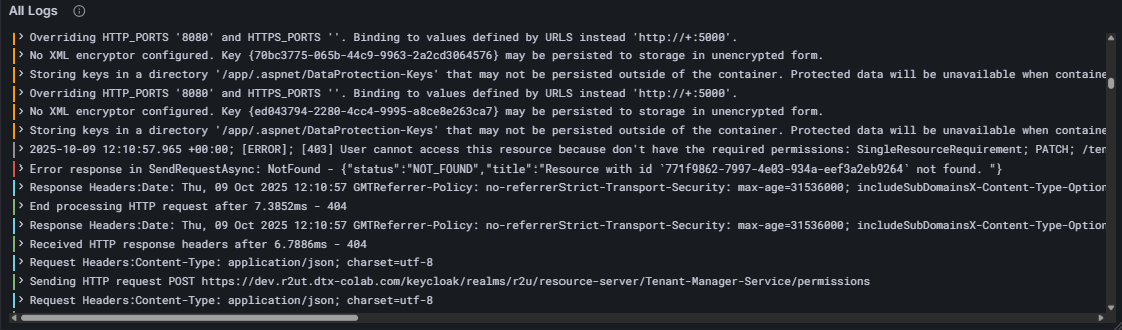
\includegraphics[width=\textwidth]{images/Grafana/all_logs_dashboard.png}
    \caption{Visão geral dos \textit{logs} estruturados do serviço \textit{TicketsManagement}.}
    \label{fig:dash-1}
\end{figure}

\textit{Transição:} Identifica-se um pico de erros ou eventos suspeitos e aplica-se filtragem 
por \texttt{service.name = TicketsManagement} e severidade (\texttt{ERROR}/\texttt{WARN}), avançando para o foco em erros.

\paragraph{2) Foco exclusivo nos erros.}

A Figura~\ref{fig:dash-2} mostra um painel dedicado exclusivamente a mensagens de erro, 
permitindo identificar \textit{endpoints} afetados, códigos HTTP e mensagens predominantes. 
Este painel acelera a identificação de falhas e reduz o \textit{MTTR} ao tornar evidentes os padrões de erro mais frequentes.

\begin{figure}[H]
    \centering
    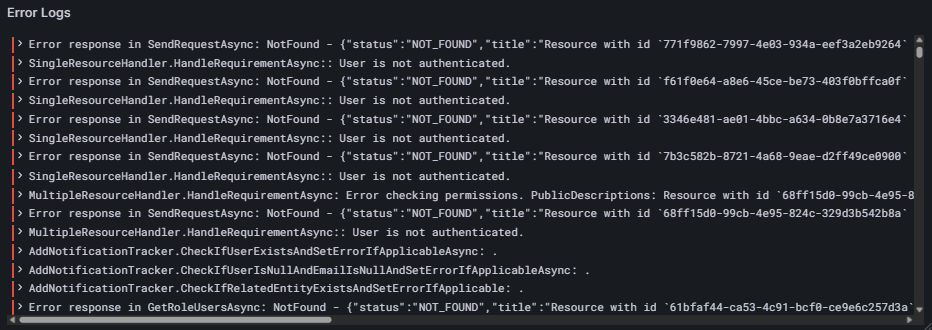
\includegraphics[width=\textwidth]{images/Grafana/error_logs_dashboard.png}
    \caption{Painel focado em \textit{logs} de erro do serviço.}
    \label{fig:dash-2}
\end{figure}

\textit{Transição:} Seleciona-se um evento concreto para análise detalhada do registo.

\paragraph{3) Expansão do registo e metadados.}

A Figura~\ref{fig:dash-3} apresenta o detalhe de um evento de \textit{log}, incluindo
\texttt{trace\_id}, \texttt{span\_id}, rota, código de estado e contexto adicional.

\begin{figure}[H]
    \centering
    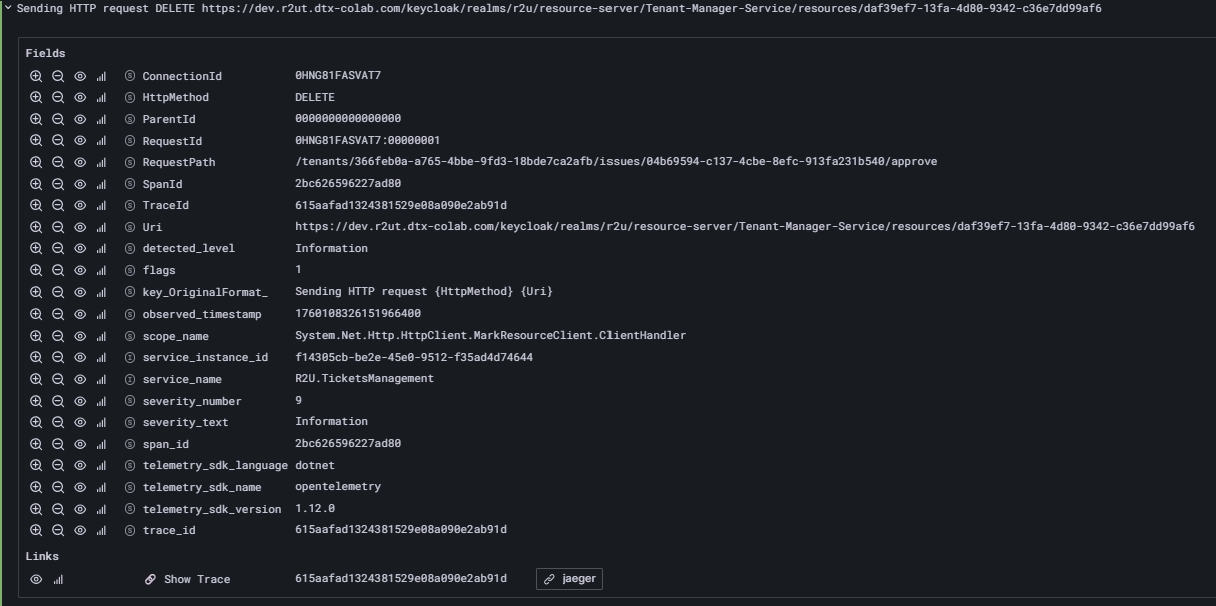
\includegraphics[width=0.9\textwidth]{images/Grafana/log_expanded.png}
    \caption{Detalhe de \textit{log} com metadados e referência direta ao trace.}
    \label{fig:dash-3}
\end{figure}

\textit{Transição:} A partir do \texttt{trace\_id}, o analista segue para o rastreamento associado.

\paragraph{4) Métricas da aplicação.}

A Figura~\ref{fig:dash-4} apresenta indicadores operacionais da API: pedidos por segundo (RPS), distribuição por códigos HTTP, latência média e percentis (p95/p99). Este painel contextualiza o erro no panorama global do serviço: variações de latência ou picos de erros tendem a refletir-se aqui.

\begin{figure}[H]
    \centering
    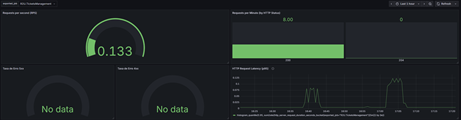
\includegraphics[width=\textwidth]{images/Grafana/metrics_dashboard.png}
    \caption{Métricas da aplicação: RPS, códigos HTTP, latência média e percentis.}
    \label{fig:dash-4}
\end{figure}

\textit{Transição.} Se houver degradação, o analista volta aos eventos e segue para o \textit{trace} para localizar gargalos. Em paralelo, valida se há limitação de recursos na infraestrutura.

\paragraph{5) Recursos da infraestrutura Kubernetes.}

A Figura~\ref{fig:dash-5} consolida métricas do cluster: utilização de CPU e memória por nó e por \textit{pod}, \textit{load average} e espaço de disco. Serve para confirmar ou excluir causas relacionadas com recursos (e.g., \textit{throttling}, saturação, \textit{out-of-memory}).

\begin{figure}[H]
    \centering
    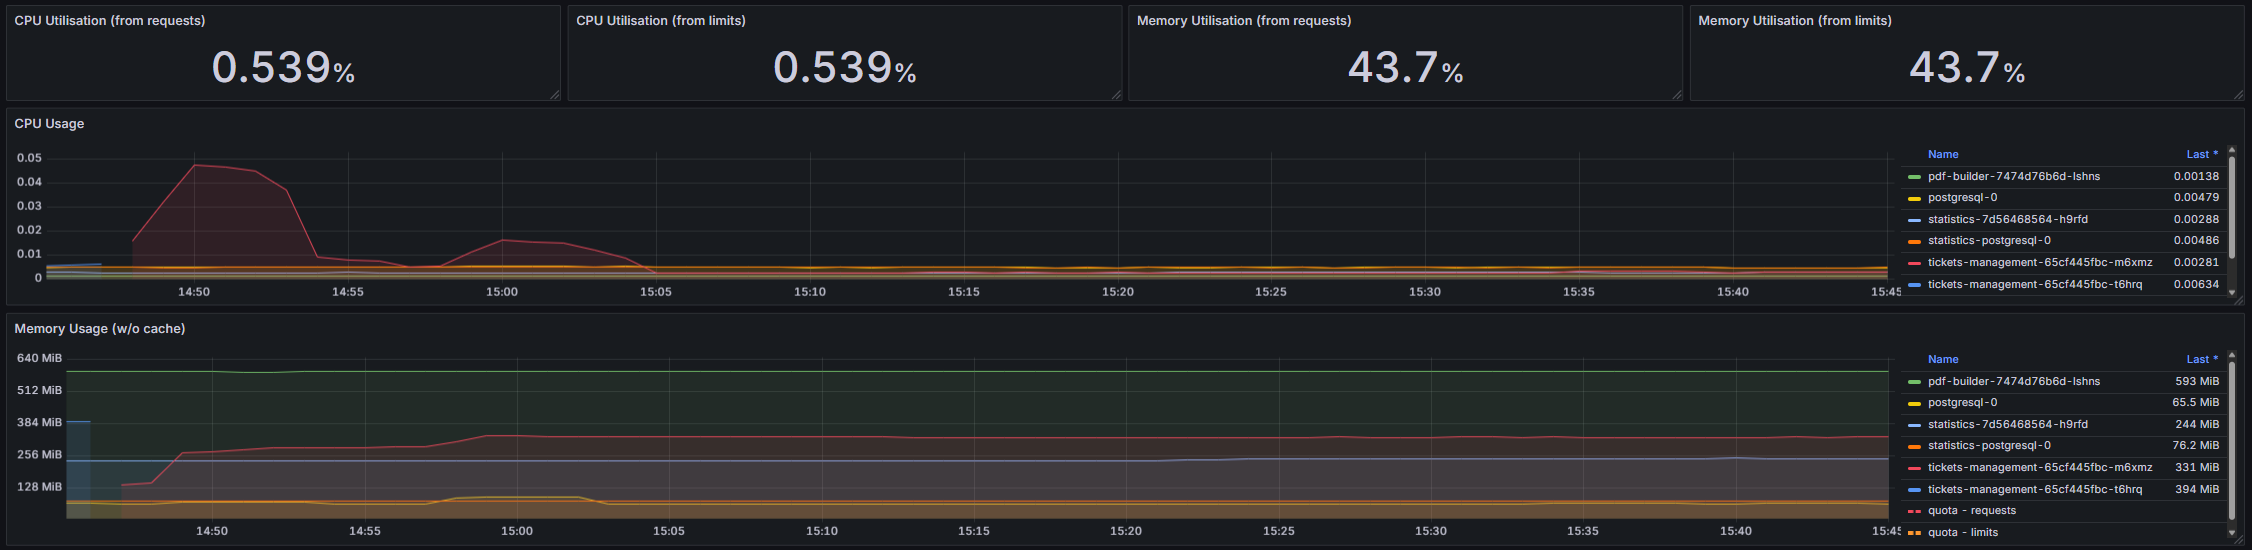
\includegraphics[width=\textwidth]{images/Grafana/cpu_memory_dashboard.png}
    \caption{Métricas de infraestrutura Kubernetes.}
    \label{fig:dash-5}
\end{figure}

 \textit{Transição.} Com os recursos estáveis, a investigação regressa ao encadeamento distribuído das chamadas para localizar a origem funcional do problema.

\paragraph{6) Rastreio distribuído.}

A Figura~\ref{fig:dash-6} ilustra um rastreamento completo associado ao incidente analisado. Observam-se as chamadas entre microsserviços, o tempo gasto em cada \textit{span} e a identificação de \textit{bottlenecks} (e.g., chamadas a \textit{databases} ou serviços externos).

\begin{figure}[H]
    \centering
    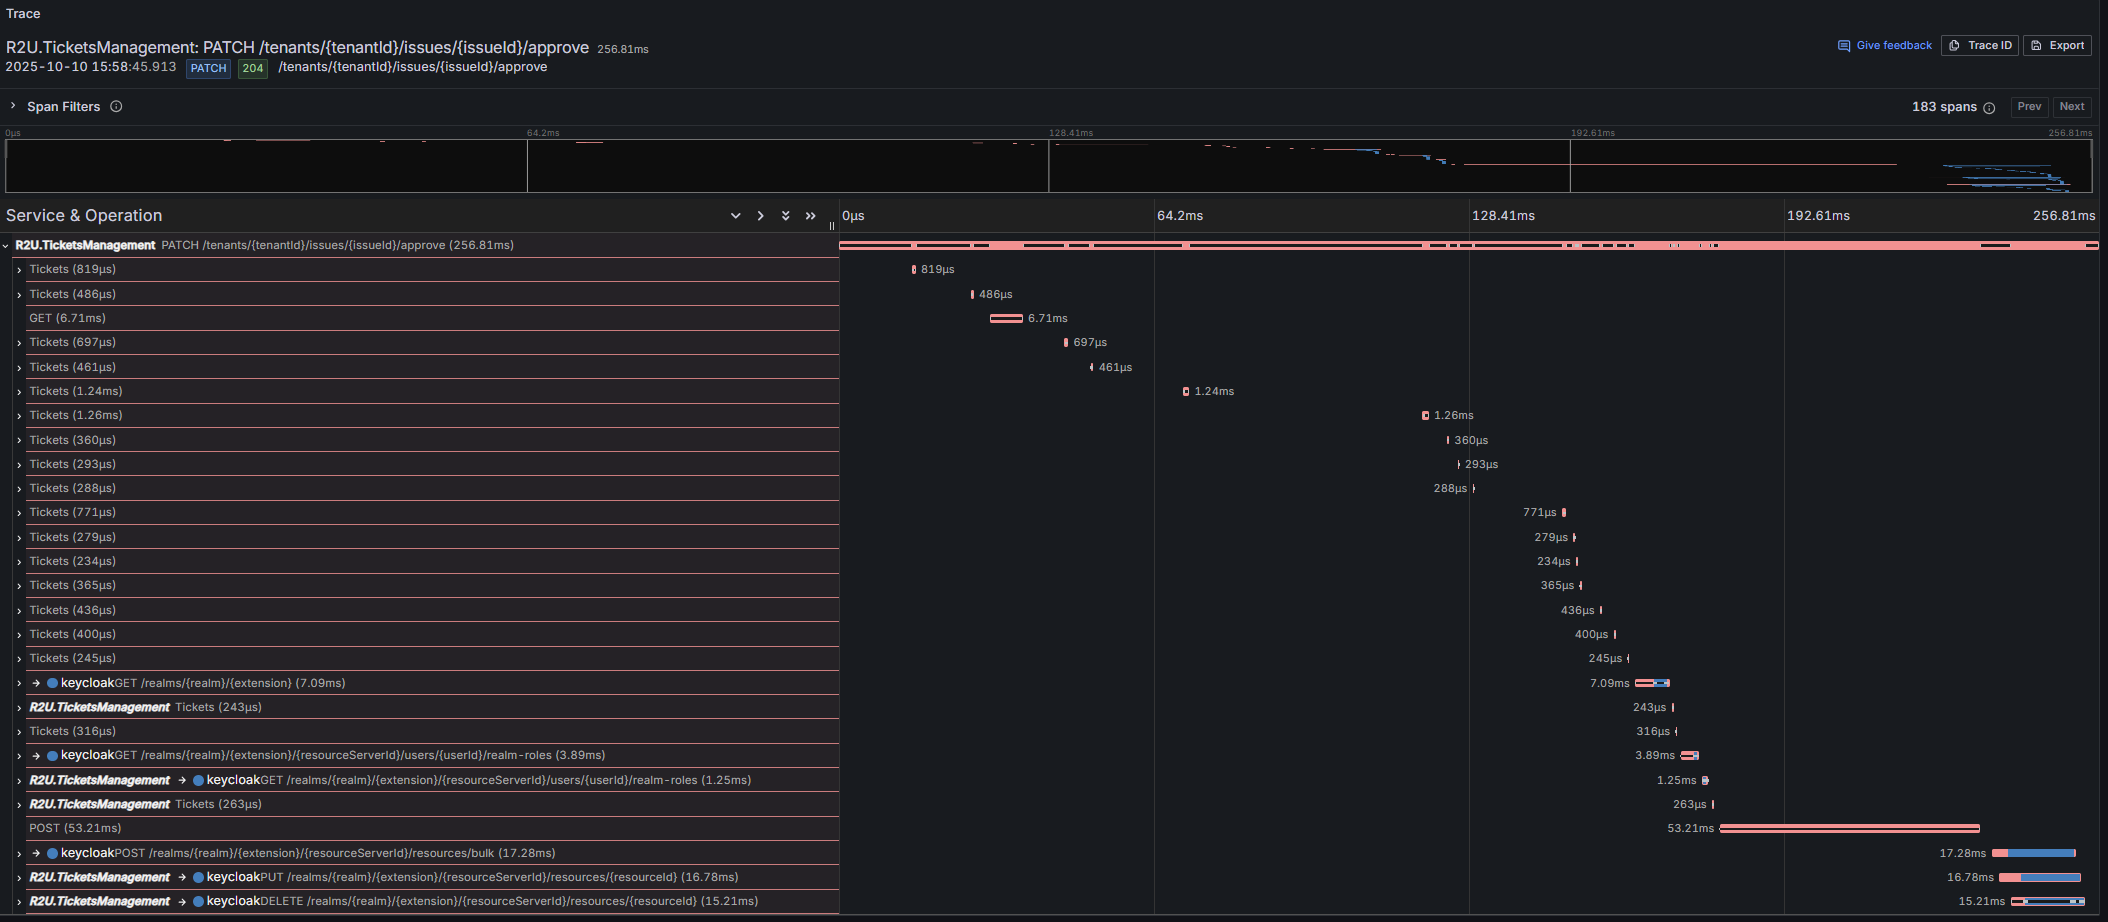
\includegraphics[width=\textwidth]{images/Grafana/trace_approve.png}
    \caption{Rastreamento distribuído associado ao evento analisado.}
    \label{fig:dash-6}
\end{figure}

\break

\subsection{Correlação entre Logs e Traces}

Um dos principais benefícios da solução implementada reside na correlação direta entre \textit{logs} 
e \textit{traces}. A Figura~\ref{fig:dash-7} apresenta um painel que liga cada registo de \textit{log} ao 
\textit{trace} correspondente, permitindo navegar rapidamente entre eventos e fluxos de execução.

\begin{figure}[H]
    \centering
    
\includegraphics[width=0.8\textwidth]{images/Grafana/trace_link_por_log.png}
    \caption{Ligação direta do \textit{log} ao \textit{trace} correspondente.}
    \label{fig:dash-7}
\end{figure}

Esta funcionalidade acelera significativamente a deteção da causa raiz de incidentes, 
uma vez que permite cruzar mensagens de erro com a linha temporal e contexto completo 
da execução distribuída.

\paragraph{Nota sobre a migração da plataforma.}
Apesar da eficácia demonstrada, importa mencionar que a plataforma R2UT encontra-se ainda 
em fase de migração gradual para Kubernetes. Assim, apenas os serviços já migrados 
emitem telemetria compatível com o modelo adotado. À medida que a migração progride, a 
monitorização será estendida a toda a plataforma, permitindo rastreamento ponta-a-ponta.

\paragraph{Síntese do fluxo analítico.}
O processo recomendado segue a sequência:

\begin{enumerate}
\item Iniciar em \textit{logs} gerais (Figura~\ref{fig:dash-1}) e identificar picos;
\item Focar erros (Figura~\ref{fig:dash-2});
\item Expandir registo e seguir o \texttt{trace\_id} (Figura~\ref{fig:dash-3});
\item Validar métricas globais (Figura~\ref{fig:dash-4});
\item Confirmar estado da infraestrutura (Figura~\ref{fig:dash-5});
\item Inspecionar \textit{trace} completo (Figura~\ref{fig:dash-6});
\item Consolidar correlação (Figura~\ref{fig:dash-7}).
\end{enumerate}

Este método reduz o tempo de análise e materializa o Grafana enquanto \textit{single pane of glass} 
para operação e diagnóstico.



% ---------------


% Para fins de demonstração e análise, os dashboards apresentados nesta secção incidem especificamente sobre o microserviço \textit{TicketsManagement}. Esta opção foi tomada com o objetivo de ilustrar o comportamento real da monitorização e dos sinais de telemetria num componente concreto da plataforma, permitindo uma leitura detalhada dos resultados e evitando dispersão analítica. 

% Embora a solução desenvolvida suporte a monitorização integral de todos os microserviços da plataforma R2UT, a inclusão simultânea de múltiplos serviços resultaria em redundância visual e conceptual, uma vez que os padrões observados --- em termos de métricas, logs e rastreamento distribuído --- são replicáveis transversalmente para os restantes componentes. Assim, optar por um serviço representativo permite privilegiar a profundidade da análise em detrimento da quantidade de informação apresentada, assegurando clareza e objetividade.

% A Figura~\ref{fig:dashboard-logs-gerais} apresenta uma visão geral dos \textit{logs} gerados pelo serviço \textit{TicketsManagement}. Este painel permite observar, em tempo real, as entradas de log estruturadas, incluindo o nível de severidade, o conteúdo textual e os metadados associados à requisição. Esta visualização é fundamental para identificar padrões de erro, eventos inesperados ou comportamentos anómalos ao longo do ciclo de execução do serviço.

% Posteriormente, a Figura~\ref{fig:dashboard-logs-erros} destaca especificamente os registos classificados como erros, facilitando a análise de falhas ocorridas no serviço. Este painel permite filtrar problemas por tipo de exceção, código HTTP devolvido e origem interna no microserviço, constituindo uma ferramenta essencial para diagnóstico e redução do \textit{Mean Time to Resolution} (MTTR).

% A Figura~\ref{fig:dashboard-aplicacao} reúne métricas operacionais da API, incluindo taxa de pedidos por segundo, latência média e distribuição temporal das requisições. Estas métricas permitem avaliar a capacidade de resposta do serviço e a sua estabilidade sob diferentes níveis de carga.

% No que respeita aos recursos da infraestrutura, a Figura~\ref{fig:dashboard-k8s} apresenta o uso de CPU e memória ao nível do \textit{pod} e do nó do cluster Kubernetes. Estas informações são essenciais para acompanhar a eficiência e o dimensionamento automático da infraestrutura, garantindo que a aplicação preserva margens adequadas de recursos.

% Por fim, a Figura~\ref{fig:dashboard-trace} ilustra um evento específico capturado pelo rastreamento distribuído, permitindo analisar a sequência de execução de uma requisição e navegar entre logs, spans e metadados associados. Esta integração facilita a correlação entre sintomas observados nos logs e a causa raiz identificada no percurso da requisição.

% ------------------

% Para efeito de apresentação e análise, os dashboards apresentados neste capítulo focam-se exclusivamente nos dados relativos ao serviço específico TicketsManagement. Embora fosse perfeitamente possível incluir visualizações de outros ser-viços da arquitetura, tal abordagem tenderia a revelar informações redundantes, uma vez que os padrões e métricas observados seriam semelhantemente aplicáveis. Assim, esta escolha visa proporcionar uma análise mais clara e exemplar, evitando a dispersão do foco e privilegiando a profundidade sobre a generalidade.

% \begin{figure}[H]
%     \centering
%     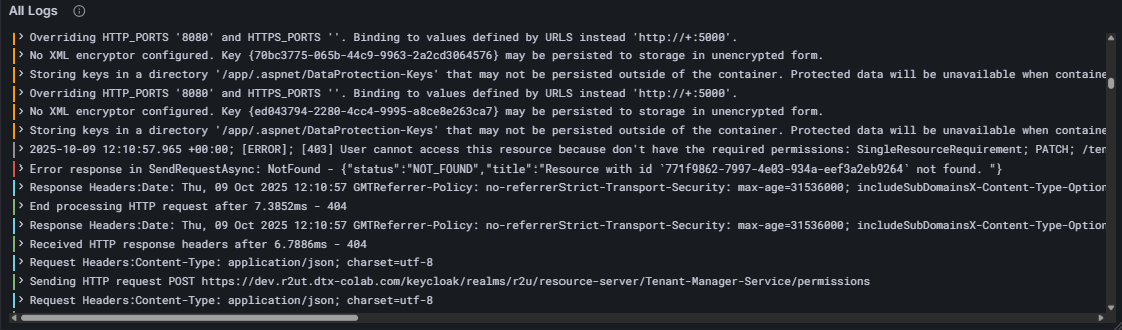
\includegraphics[width=1\textwidth]{images/Grafana/all_logs_dashboard.png}
%     \caption{Painel global de Logs}
%     % \label{fig:digital_twin}
% \end{figure}

% \begin{figure}[H]
%     \centering
%     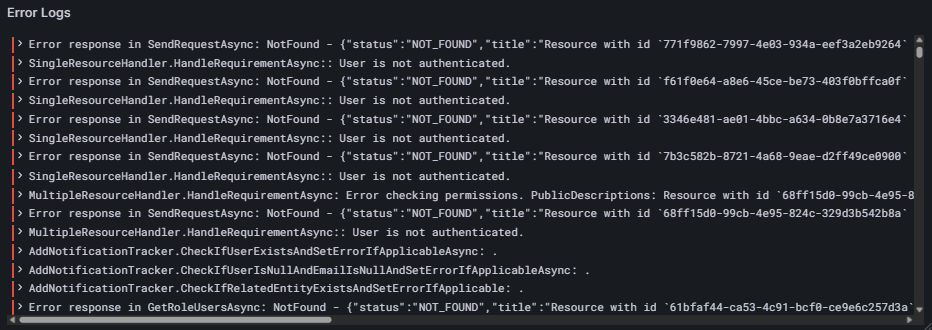
\includegraphics[width=1\textwidth]{images/Grafana/error_logs_dashboard.png}
%     \caption{Painel de Logs de Erro}
%     % \label{fig:digital_twin}
% \end{figure}

% \begin{figure}[H]
%     \centering
%     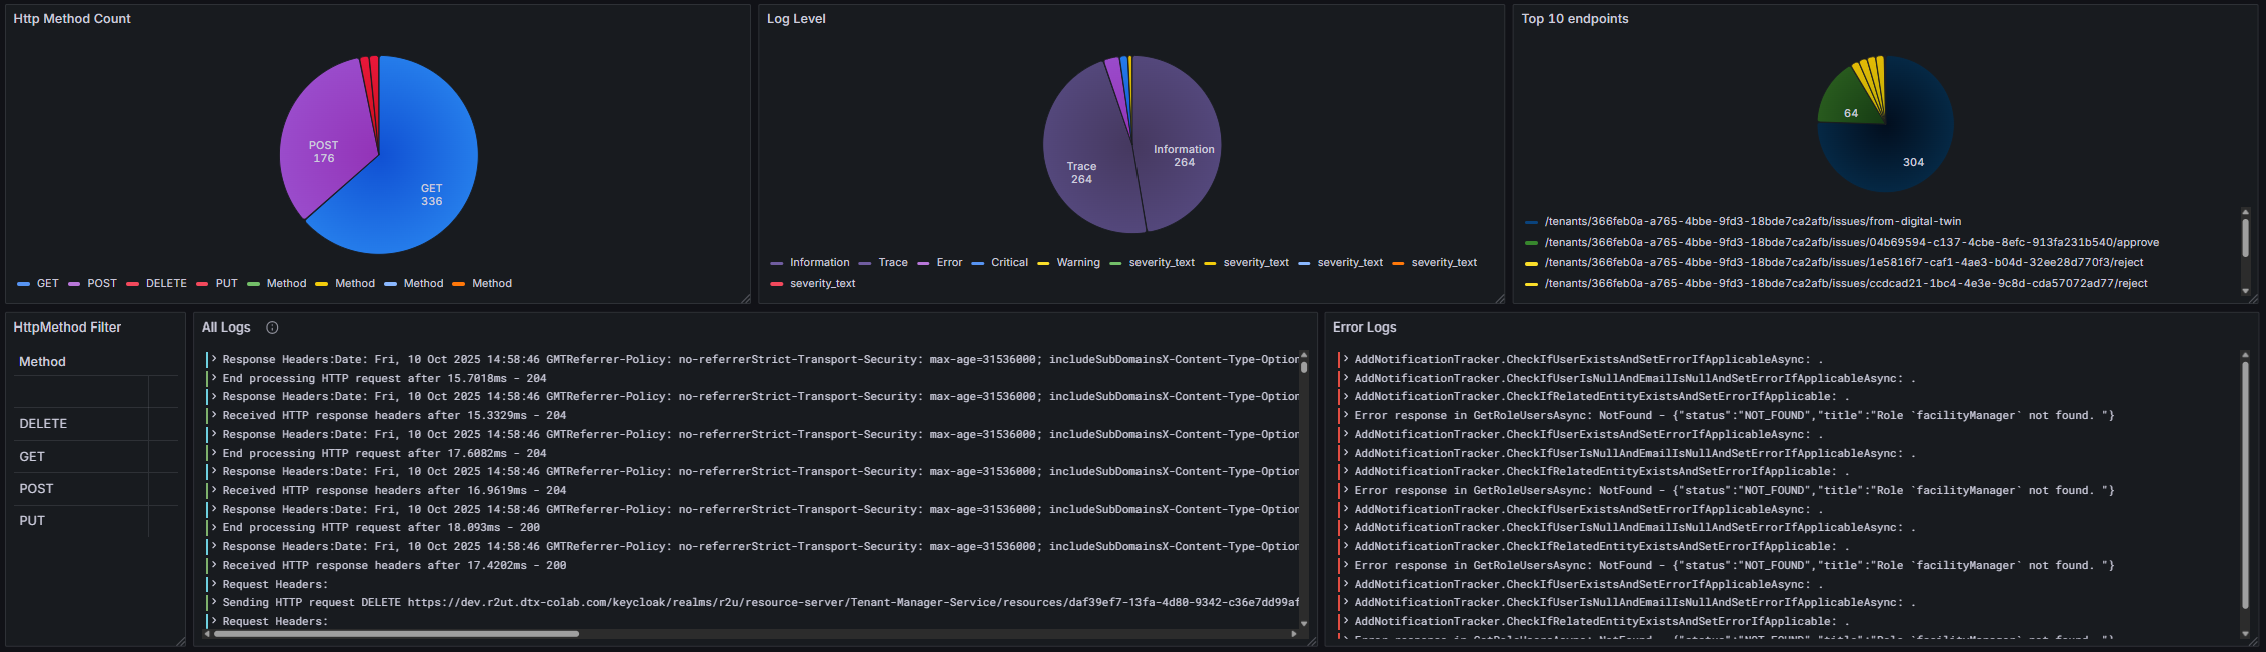
\includegraphics[width=1\textwidth]{images/Grafana/dashboard.png}
%     \caption{\textit{Dashboard} de \textit{Logs}}
%     % \label{fig:digital_twin}
% \end{figure}

% \begin{figure}[H]
%     \centering
%     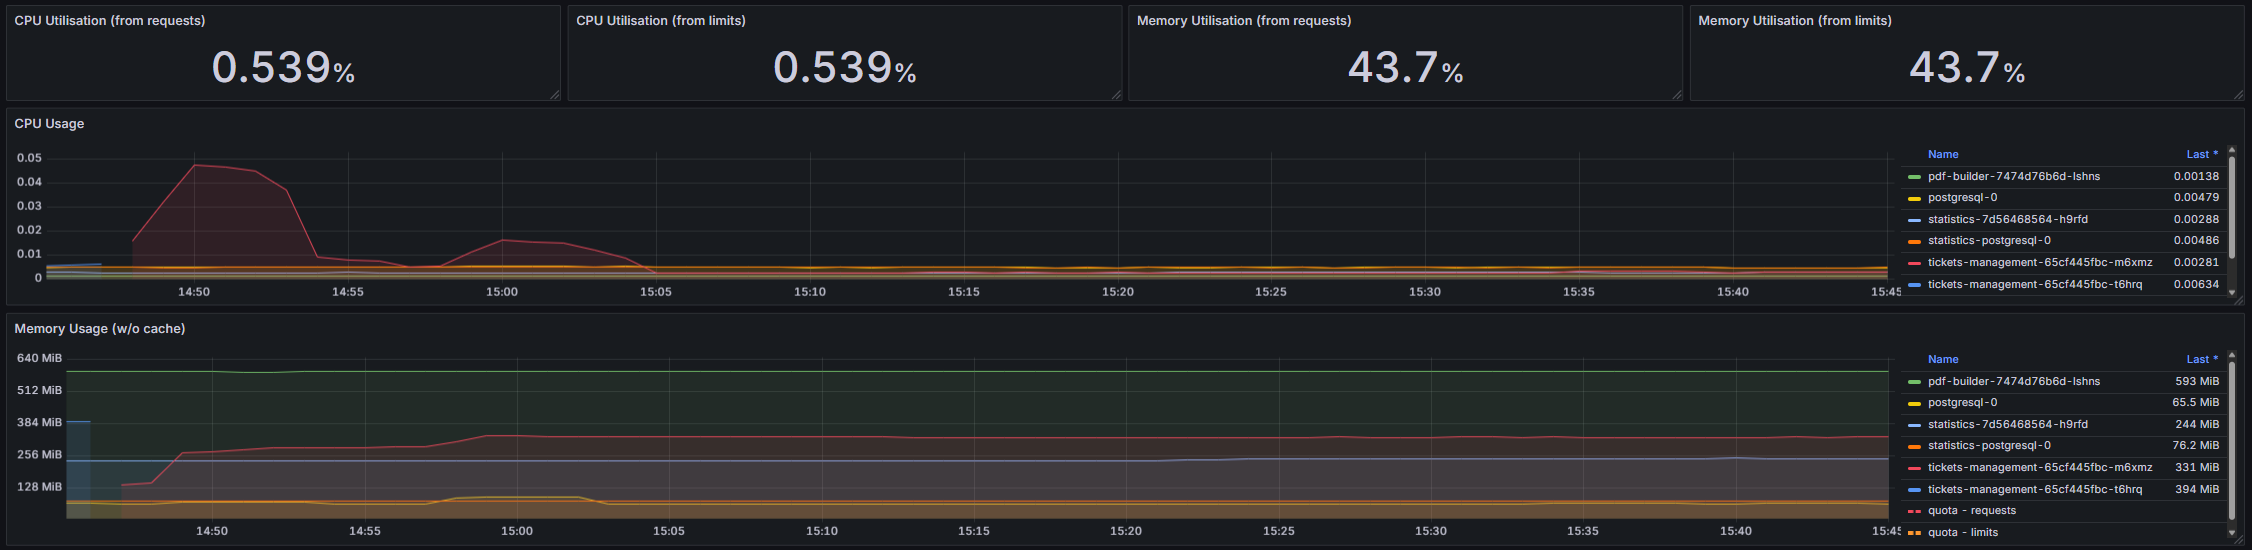
\includegraphics[width=1\textwidth]{images/Grafana/cpu_memory_dashboard.png}
%     \caption{Uso de CPU e Memória}
%     % \label{fig:digital_twin}
% \end{figure}

% \begin{figure}[H]
%     \centering
%     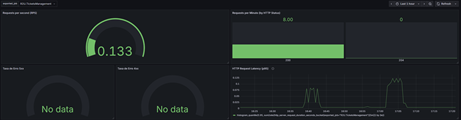
\includegraphics[width=1\textwidth]{images/Grafana/metrics_dashboard.png}
%     \caption{Dashboard de metricas: p95, Taxa de Erro, Pedidos por segundo}
%     % \label{fig:digital_twin}
% \end{figure}

% \section{Correlação entre Logs e Traces}

% Um dos principais ganhos trazidos pelo Grafana é a correlação direta entre logs e traces. Com um dashboard dedicado, foi possível implementar múltiplos filtros, incluindo o \texttt{service\_name}, que permitem visualizar os logs emitidos por diferentes serviços e vinculá-los diretamente às requisições (traces) correspondentes que os originaram.

% Cada entrada de log disponibiliza um link direto para o trace associado, simplificando significativamente a depuração e o diagnóstico de problemas. Este recurso proporciona uma visão holística do estado do sistema e das suas interações, facilitando a identificação rápida de causas de falhas ou degradação do serviço.

% \begin{figure}[H]
%     \centering
%     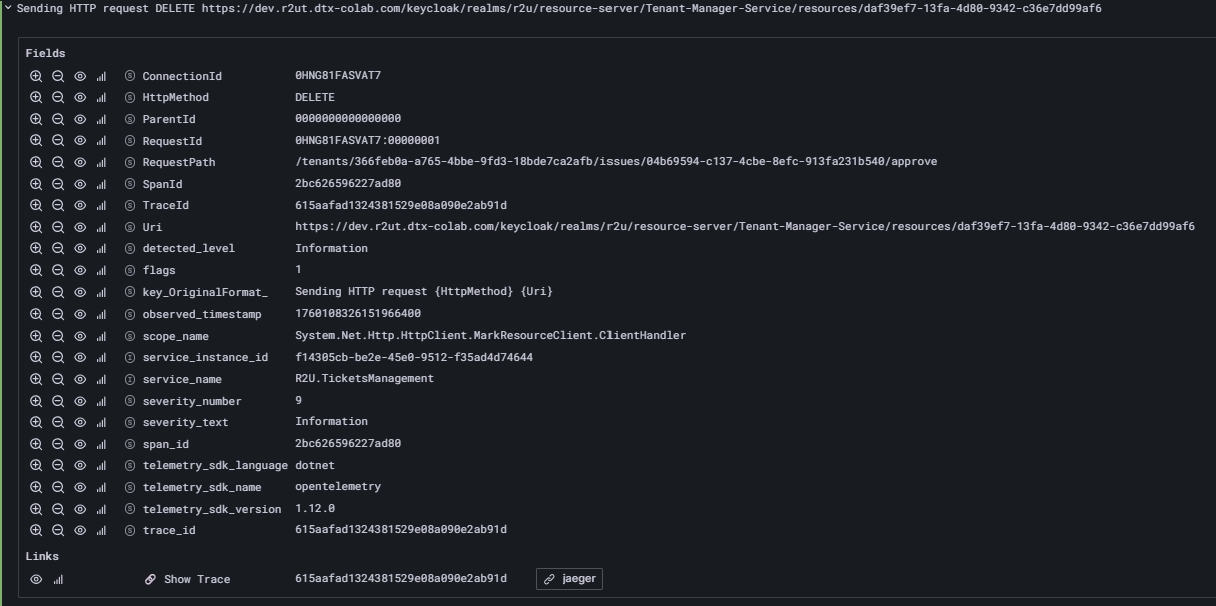
\includegraphics[width=1\textwidth]{images/Grafana/log_expanded.png}
%     \caption{Log: Correlação Log e Trace}
%     % \label{fig:digital_twin}
% \end{figure}

% \begin{figure}[H]
%     \centering
%     
\includegraphics[width=1\textwidth]{images/Grafana/trace link por log.png}
%     \caption{Link para Trace}
%     % \label{fig:digital_twin}
% \end{figure}

% \begin{figure}[h]
%     \centering
%     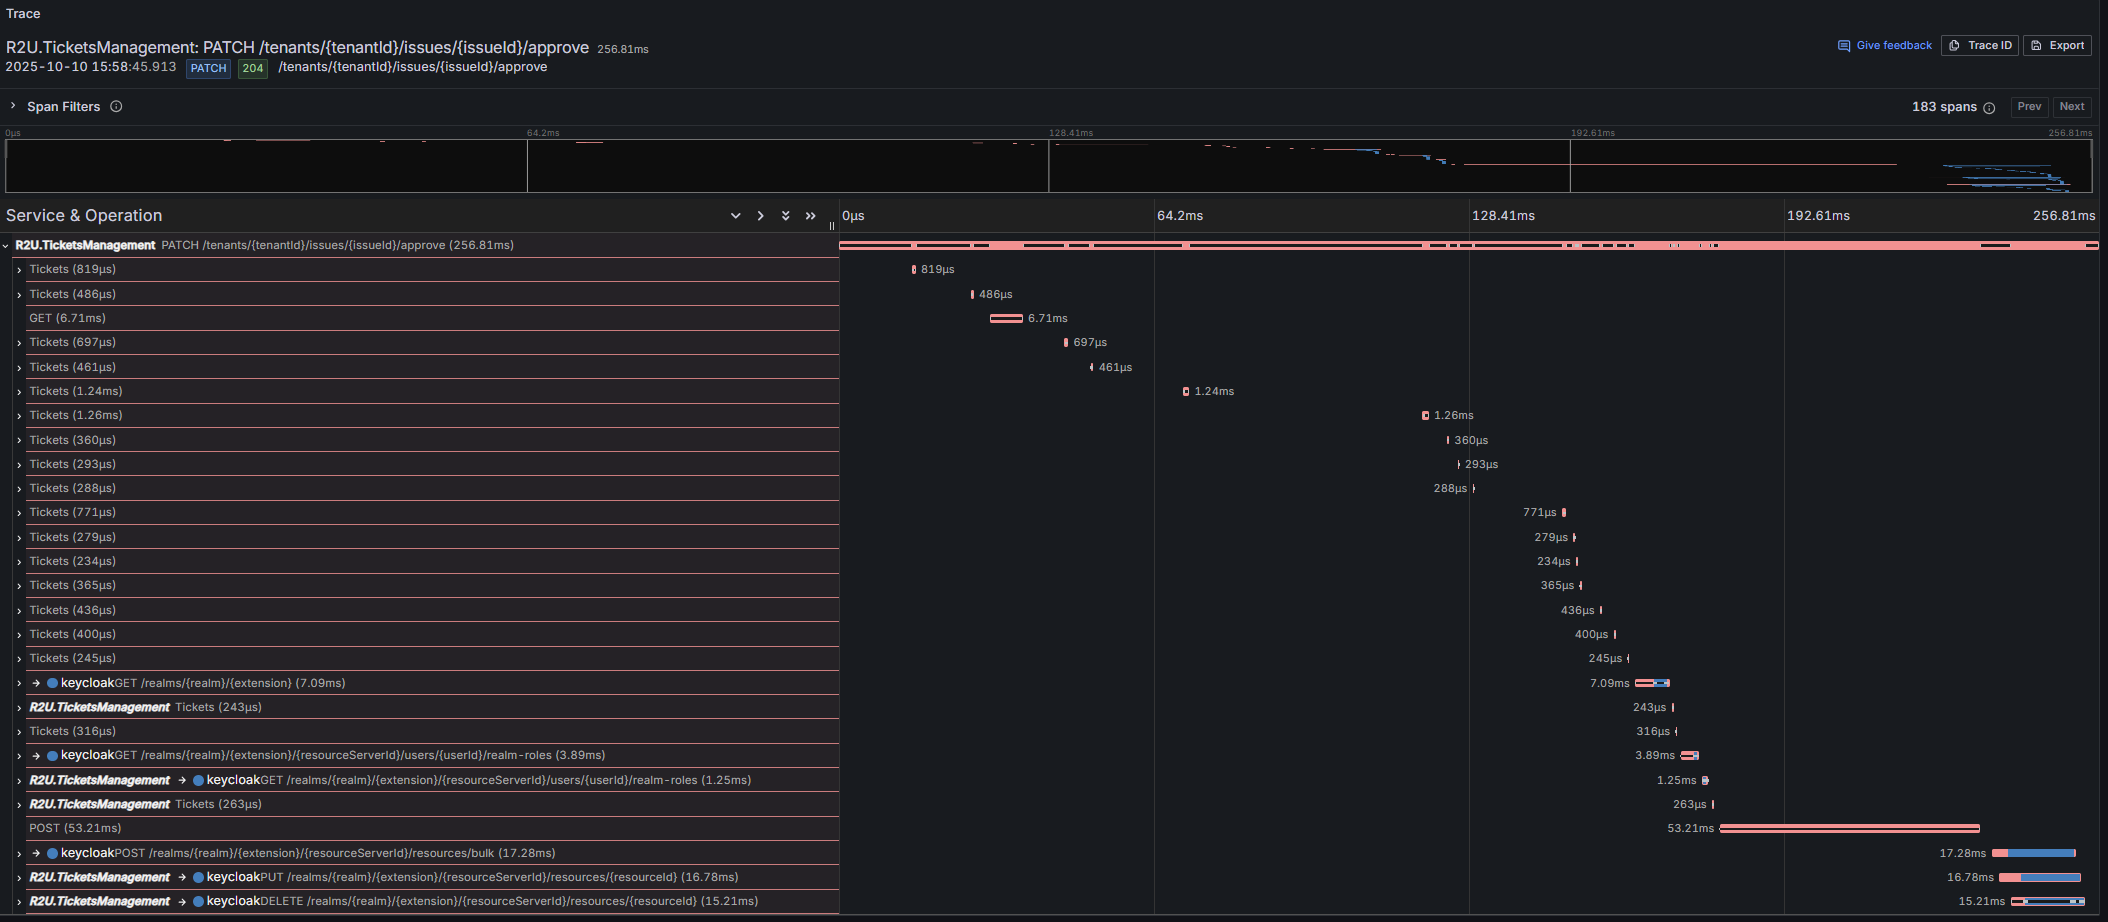
\includegraphics[width=1\textwidth]{images/Grafana/trace_approve.png}
%     \caption{Trace: Correlação Log e Trace}
%     % \label{fig:digital_twin}
% \end{figure}

\section{Alertas}

todo: falar um pouco sobre os alertas, ainda nao implementados, mas de configuracao muito simples